% main2.tex -- revision addressing the supervisor review (structure, references,
% figures, abstract/introduction story, model name, comparison + ablation studies).
% The original manuscript is untouched in main.tex.
\documentclass[conference]{IEEEtran}
\usepackage{cite}
\usepackage{amsmath,amssymb}
\usepackage{graphicx,booktabs,array}
\usepackage{balance}
\usepackage{xcolor}
\usepackage[hidelinks]{hyperref}
\graphicspath{{figures/}{refined_figures/}}

% ---- Model name (High-flow Attention and Representation Transformer Network).
\newcommand{\model}{HART-Net}
\newcommand{\bce}{N5\_bce}

% ---- Blind review switch: \blindtrue hides authors (double-blind),
%      \blindfalse shows them (single-blind). Check the venue's rules.
\newif\ifblind
\blindtrue

\begin{document}
\title{\model{}: A Terrain-Conditioned High-flow Attention and Representation Transformer for Next-Day River Forecasting in Sri Lanka}

\ifblind
\author{\IEEEauthorblockN{Anonymous Authors}
\IEEEauthorblockA{Affiliation withheld for double-blind review}}
\else
\author{%
\IEEEauthorblockN{%
Heshan Nethmina, Ranuga Weerasekara, Dinithi Navodya, Manuja Ranathunga,\\
and Vinma Wettasinghe}
\IEEEauthorblockA{%
Department of Computer Science \& Engineering\\
University of Moratuwa, Moratuwa, Sri Lanka\\
\texttt{\{heshann.23, ranugaw.23, dinithin.23, manujar.23, vinmaw.23\}@cse.mrt.ac.lk}}}
\fi
\maketitle

%% =====================================================================
\begin{abstract}
Monsoon floods recur across Sri Lanka, yet data-driven forecasting studies in
the country mostly cover a single station and few events, and report accuracy,
which hides poor detection of rare floods. A national model is difficult
because high-flow days are rare and deep networks often trail tree models on
tabular weather and river data. Our first spatio-temporal graph network showed
this gap, and diagnosis traced it to a weak numerical input layer. We therefore
propose \model{} (High-flow Attention and Representation Transformer Network)
for next-day high-flow prediction. \model{} embeds every input value with
periodic numerical embeddings, models two weeks of history with a temporal
transformer, lets variables interact through cross-feature attention, and
adapts one shared network to each location's terrain through feature-wise
linear modulation, trained with a multi-task objective and deployed as a
calibrated deep ensemble. On an open dataset built from public reanalysis for
51 locations in 16 basins over 22 years, evaluated on held-out years
2021--2024, \model{} achieves an average precision (AP) of 0.836, a 13\%
improvement over our spatio-temporal graph network and 11\% over its
graph-augmented variant, while cutting the false-alarm ratio by about 60\%. It
outperforms persistence, the operational discharge-percentile rule and a compact
neural ensemble at every forecast horizon and at flood onset, matches a
gradient-boosted tree at one day while exceeding it at longer horizons and
onset with one-third fewer false alarms, and delivers highly reliable
probabilities (expected calibration error 0.0016). Ablations
show that periodic embeddings alone raise AP by 25\% and terrain conditioning
cuts false alarms by nearly two-thirds.
\end{abstract}

\begin{IEEEkeywords}
flood forecasting, transformer, numerical embeddings, feature-wise linear
modulation, probability calibration, Sri Lanka
\end{IEEEkeywords}

%% =====================================================================
\section{Introduction}
Floods are Sri Lanka's most frequent natural hazard. The south-west monsoon
brings repeated flooding to the Kelani, Kalu, Gin and Nilwala basins, while the
north-east monsoon floods the dry-zone basins of the east and north. A useful
early-warning model must therefore work across contrasting climates and river
sizes, and it must say not only \emph{whether} a river will rise but
\emph{how likely} that is, so that warnings can be trusted.

Deep learning has transformed hydrological modelling. Recurrent networks learn
rainfall--runoff behaviour from data \cite{kratzert2018,kratzert2019}, and
large-scale systems now forecast extreme floods in ungauged basins
\cite{nearing2024}. In Sri Lanka, however, data-driven studies remain local:
they model a single station or district, evaluate on a handful of flood events,
and often report accuracy, which is misleading when almost every day is a
non-flood day \cite{saubhagya2025,thilakarathne2017}. There is no national,
openly reproducible deep-learning benchmark for the country.

Two technical obstacles stand in the way. First, high-flow days are rare, so a
model can look accurate while missing most of them; ranking quality,
calibration and false alarms must be measured instead. Second, the inputs are
tabular: rainfall totals, soil wetness and discharge statistics. On such data,
gradient-boosted trees frequently outperform deep networks
\cite{grinsztajn2022,ke2017}. Our first model, a spatio-temporal graph network
that combined a recurrent encoder with river-network attention, reproduced this
gap. Diagnosing it, we found that the network's weakness lay in how it read
individual numbers, not in its depth or its spatial structure.

This motivates \model{}, the High-flow Attention and Representation Transformer
Network. Instead of feeding raw scalars to the network, we embed
every input value with periodic numerical embeddings \cite{gorishniy2022}, which
let a network form sharp, threshold-like responses similar to tree splits. A
temporal transformer \cite{vaswani2017} then reads two weeks of history and can
attend directly to the day heavy rain fell, while a cross-feature attention
branch, in the spirit of feature-tokenised tabular transformers
\cite{gorishniy2021}, lets variables interact. Because the same rainfall
produces different responses at different locations, a feature-wise linear
modulation (FiLM) layer \cite{perez2018} conditions one shared network on each
location's terrain, climate zone and river position. A multi-task objective
supervises several horizons and flood onset together, and a deep ensemble with
temperature scaling turns the outputs into calibrated probabilities
\cite{lakshminarayanan2017,guo2017}. The design is related to the Temporal
Fusion Transformer \cite{lim2021}, which also conditions temporal attention on
static covariates, but replaces its recurrent and variable-selection components
with numerical embeddings and FiLM, and targets calibrated classification of
rare events.

The main contributions of this work are:
\begin{itemize}
\item \model{}, a terrain-conditioned transformer that combines periodic
numerical embeddings, temporal and cross-feature attention, FiLM conditioning
and a calibrated ensemble for next-day high-flow forecasting.
\item An open, leakage-controlled national dataset built from public reanalysis
sources, with chronological splits and training-period-only thresholds.
\item A comparison study against operational rules, a gradient-boosted tree and
alternative graph-based and compact neural architectures, and an ablation study that isolates the
effect of each architectural and training choice.
\end{itemize}

%% =====================================================================
\section{Related Work}
\subsection{Neural hydrological forecasting}
Long short-term memory (LSTM) networks \cite{hochreiter1997} established that
river response can be learned from meteorological sequences
\cite{kratzert2018}; entity-aware variants use static catchment attributes to
control the recurrent state \cite{kratzert2019}. Global operational systems now
extend such models to ungauged basins \cite{nearing2024}. Reviews of
machine-learning flood prediction highlight data scarcity and evaluation
practice as recurring weaknesses \cite{mosavi2018}. In Sri Lanka, Saubhagya
\emph{et al.} combine a bidirectional LSTM with regression to forecast water
level at Ratnapura in the Kalu basin \cite{saubhagya2025}; Thilakarathne and
Premachandra forecast monthly floods in the North Central Province with ARIMA
and a small neural network \cite{thilakarathne2017}; and hydraulic modelling
has mapped flood hazard on the lower Kelani \cite{gunasekara2008}. These
studies differ from ours in target, horizon and scale, so their scores are not
directly comparable.

\subsection{Deep learning for tabular and multivariate time series}
Tree ensembles remain strong on tabular data \cite{grinsztajn2022,ke2017}.
FT-Transformer tokenises each feature and applies self-attention
\cite{gorishniy2021}, and periodic numerical embeddings close much of the
remaining gap to trees \cite{gorishniy2022}, related to Fourier feature mappings
\cite{tancik2020}. The Temporal Fusion Transformer couples recurrent layers,
self-attention, gating and static covariate encoders for multi-horizon
forecasting \cite{lim2021}. \model{} adopts the embedding and tokenisation ideas
but uses a pure transformer encoder with a classification token \cite{devlin2019}.

\subsection{Conditioning and spatial structure}
FiLM conditions a representation through learned feature-wise scale and shift
\cite{perez2018}. River graphs offer an alternative way to inject hydrological
structure, but Kirschstein and Sun found that river topology did not improve
their neural forecasts \cite{kirschstein2024}; we test this question directly.

\subsection{Calibration and evaluation}
Focal loss down-weights easy examples \cite{lin2017}. Deep ensembles and
temperature scaling are established tools for probability quality
\cite{lakshminarayanan2017,guo2017,naeini2015}. Under rare positives,
precision--recall analysis is more informative than accuracy or ROC curves
\cite{saito2015}, and forecast verification uses the Brier score and
contingency scores \cite{brier1950,jolliffe2012}. Temporally dependent data
require chronological evaluation to avoid leakage \cite{roberts2017,kapoor2023}.

%% =====================================================================
\section{Data and Problem Formulation}
\label{sec:data}
\subsection{Locations and sources}
The dataset covers $N$ river locations in 16 basins or areas: wet-zone,
dry-zone and intermediate-zone sites placed along major rivers, from upstream
reaches to river mouths (Fig.~\ref{fig:map}). These are modelling locations
rather than measured gauges. Daily meteorology and soil wetness come from NASA
POWER \cite{power}; precipitation preferentially comes from ERA5-Land
\cite{munoz2021} via the Open-Meteo archive, with POWER as a fallback; and
river discharge comes from the GloFAS reanalysis \cite{harrigan2020} via the
Open-Meteo Flood API \cite{openmeteo}. All sources are public and require no
access key.

\begin{figure}[t]
\centering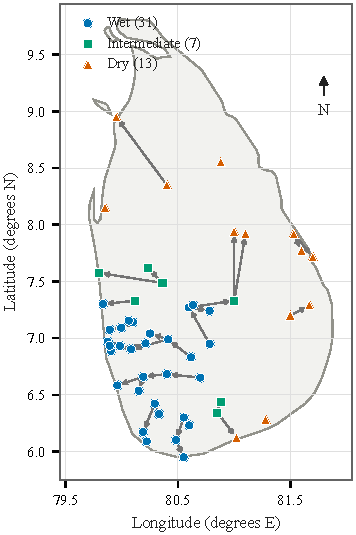
\includegraphics[width=.78\linewidth]{fig_study_area.pdf}
\caption{Study locations and curated upstream-to-downstream links, coloured by
climatic zone. Country outline: Natural Earth.}
\label{fig:map}
\end{figure}

\subsection{Features and preprocessing}
Each location has $F$ dynamic variables per day: rainfall and antecedent-rainfall
indices, temperature, humidity, wind and radiation, soil wetness and its
anomaly, and discharge statistics (changes, rolling means, seasonal anomaly and
empirical percentile). It also has $S$ static attributes: elevation, a drainage
proxy (log mean training discharge), one-hot climatic zone and one-hot river
position. Heavy-tailed variables receive a signed $\log(1+|x|)$ transform; all
variables are standardised with statistics fitted on the training period only,
and missing values are set to the training mean.

\subsection{Targets and episodes}
Let $Q_{n,t}$ be discharge at location $n$ on day $t$. The high-flow state and
the primary next-day target are defined in \eqref{eq:thresholds}:
\begin{align}
\tau_n &= \operatorname{quantile}_{0.98}\{Q_{n,t}:t\le\text{2017-12-31}\},\\
s_{n,t} &= \mathbf{1}[Q_{n,t}\ge\tau_n],\qquad y^{(1)}_{n,t}=s_{n,t+1}.
\label{eq:thresholds}
\end{align}
Auxiliary targets mark any exceedance within two and three days,
$y^{(h)}_{n,t}=\max_{k\le h}s_{n,t+k}$, and next-day onset,
$y^{(o)}_{n,t}=(1-s_{n,t})s_{n,t+1}$; two regression targets are the next-day
discharge percentile and the three-day maximum discharge z-score. Positive state
days separated by at most two days form a node-level \emph{episode}. The
percentile threshold defines relative high flow, not observed inundation.

\subsection{Chronological split}
Training uses 2003--2017, validation 2018--2020 and testing 2021--2024. Because
neighbouring days are nearly identical, random splits leak information; all
thresholds, climatologies and normalisation statistics are therefore fitted on
the training years only. Fig.~\ref{fig:episodes} shows the episode catalogue
across the three periods.

\begin{figure}[t]
\centering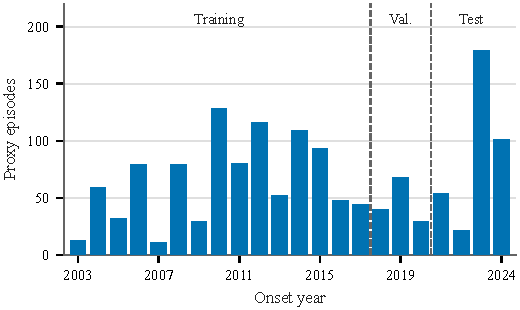
\includegraphics[width=\linewidth]{fig_episode_profile.pdf}
\caption{Annual counts of node-level high-flow episodes, with the training,
validation and test periods marked.}
\label{fig:episodes}
\end{figure}

%% =====================================================================
\section{Model Architecture}
\label{sec:method}
Fig.~\ref{fig:architecture} summarises \model{}. For location $n$ and issue day
$t$, the input is the matrix $X_{n,t}\in\mathbb{R}^{L\times F}$ of the last $L$
days. Locations are folded into the batch, so one shared network processes
every location independently.

\begin{figure}[t]
\centering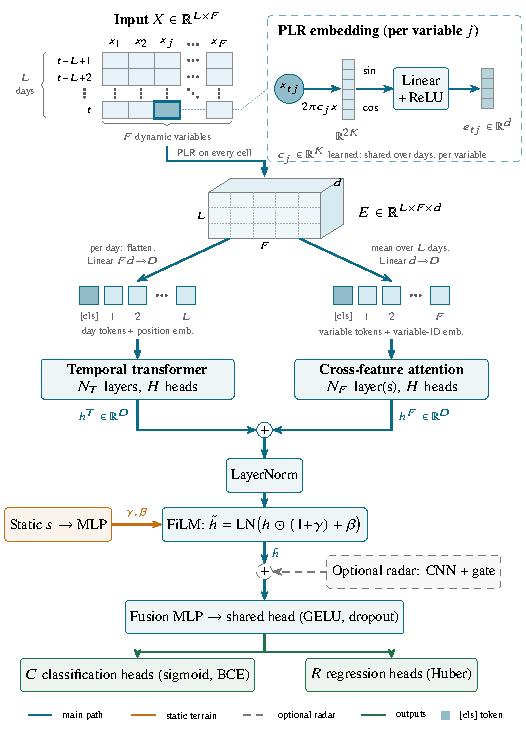
\includegraphics[width=\linewidth]{fig3_architecture.pdf}
\caption{\model{} architecture. Each input value is embedded by a PLR module;
a temporal transformer over day tokens and a cross-feature attention branch over
variable tokens are merged, conditioned on static attributes through FiLM,
optionally fused with radar features, and decoded into $C$ classification and
$R$ regression outputs. Symbol values are given in Table~\ref{tab:settings}.}
\label{fig:architecture}
\end{figure}

\subsection{Periodic numerical embedding}
Each scalar $x$ of variable $j$ is mapped to $d$ values by a
periodic--linear--ReLU (PLR) embedding \cite{gorishniy2022}:
\begin{equation}
\mathbf{e}_j(x)=\operatorname{ReLU}\!\left(
\mathbf{W}_j[\sin(2\pi\mathbf{c}_j x)\Vert\cos(2\pi\mathbf{c}_j x)]+\mathbf{b}_j\right),
\label{eq:plr}
\end{equation}
where $\mathbf{c}_j\in\mathbb{R}^{K}$ are learned frequencies. Parameters are
separate for each variable and shared across days, so the input matrix becomes a
tensor $E\in\mathbb{R}^{L\times F\times d}$. The periodic basis lets the network
represent sharp, threshold-like responses to individual variables.

\subsection{Temporal and cross-feature attention}
In the temporal branch, each day's $F\times d$ embeddings are flattened and
projected to a width-$D$ token. A learned classification token and position
embeddings are added, and $N_T$ pre-layer-normalised transformer layers
\cite{vaswani2017,xiong2020} with $H$ heads, GELU activations
\cite{hendrycks2016} and dropout produce the summary $\mathbf{h}^{T}$. In the
cross-feature branch, embeddings are averaged over the $L$ days, projected to
width $D$ and tagged with a learned variable identity; $N_F$ attention layers
over these variable tokens produce $\mathbf{h}^{F}$. The branches merge as
\begin{equation}
\mathbf{h}=\operatorname{LN}(\mathbf{h}^{T}+\mathbf{h}^{F}),
\label{eq:merge}
\end{equation}
where $\operatorname{LN}$ is layer normalisation \cite{ba2016}.

\subsection{Terrain conditioning with FiLM}
A small MLP maps the static vector $\mathbf{s}_n\in\mathbb{R}^{S}$ to a scale
$\gamma_n$ and shift $\beta_n$ \cite{perez2018}:
\begin{equation}
\widetilde{\mathbf{h}}=\operatorname{LN}[\mathbf{h}\odot(1+\gamma_n)+\beta_n].
\label{eq:film}
\end{equation}
The final MLP layer is zero-initialised, so conditioning starts neutral and the
model learns how strongly terrain should modify its state.

\subsection{Optional radar fusion}
For experiments with Sentinel-1 imagery \cite{torres2012}, a ResNet-style CNN
\cite{he2016} encodes two-channel VV/VH chips into $\mathbf{v}$, and a learned
gate adds them only when an image exists:
\begin{align}
\mathbf{g}&=\sigma\{\operatorname{MLP}[\widetilde{\mathbf{h}}\Vert\mathbf{v}\Vert m\Vert(a/30)]\},\\
\mathbf{h}^{S}&=\operatorname{LN}(\widetilde{\mathbf{h}}+m\,\mathbf{g}\odot\mathbf{W}_v\mathbf{v}),
\label{eq:radar}
\end{align}
where $m$ indicates image presence and $a$ its age in days. The gate bias starts
at $-3$, so the branch starts nearly closed.

\subsection{Multi-task objective}
A fusion MLP and shared head produce $C$ classification logits and $R$
regression outputs. The loss is
\begin{equation}
\mathcal{L}=\sum_{k=1}^{C} w_k\,\mathrm{BCE}_k+\lambda\,\mathrm{Huber},
\label{eq:loss}
\end{equation}
with masked binary cross-entropy for the next-day, two-day, three-day and onset
heads and the Huber loss \cite{huber1964} for the regressions. We also evaluate
focal loss \cite{lin2017} combined with a label-confidence weight that lowers
the influence of days near the threshold.

\subsection{Ensemble and calibration}
Five members trained with different seeds are averaged in probability space and
calibrated by temperature scaling \cite{lakshminarayanan2017,guo2017}:
\begin{equation}
\bar p=\frac{1}{M}\sum_{k=1}^{M}p_k,\qquad
p_{\mathrm{cal}}=\sigma\!\left[\frac{\operatorname{logit}(\bar p)}{T}\right],
\label{eq:calibration}
\end{equation}
with $T$ fitted on validation data. The alarm threshold maximises validation F1
and is frozen for testing.

%% =====================================================================
\section{Experimental Setup}
\subsection{Implementation}
Table~\ref{tab:settings} lists the configuration. Models are implemented in
PyTorch \cite{paszke2019} and trained with AdamW \cite{loshchilov2019}, five
warm-up epochs and a cosine schedule, gradient clipping and early stopping on
validation episode-level average precision, on a single NVIDIA T4 GPU.

\begin{table}[t]
\caption{Configuration of \model{}.}
\label{tab:settings}
\centering\footnotesize
\begin{tabular}{@{}p{0.50\columnwidth}p{0.42\columnwidth}@{}}
\toprule
Setting & Value \\
\midrule
History $L$; dynamic $F$; static $S$ & 14 days; 33; 9 \\
PLR frequencies $K$; embedding $d$ & 8; 8 \\
Width $D$; heads $H$; layers $N_T$/$N_F$ & 128; 4; 3/1 \\
Fusion / head widths & 192 / 256 \\
Outputs $C$ / $R$; loss weights $w$; $\lambda$ & 4 / 2; (1, .3, .3, .5); 0.2 \\
Optimiser; learning rate; weight decay & AdamW; $10^{-3}$; $10^{-4}$ \\
Batch; max epochs; patience & 32 days; 60; 10 \\
Ensemble size $M$ & 5 \\
\bottomrule
\end{tabular}
\end{table}

\subsection{Baselines and compared models}
We compare against two operational rules, a gradient-boosted tree and three
alternative neural architectures that we developed: (i) \emph{persistence},
which predicts tomorrow's state as today's; (ii) a \emph{discharge-percentile
rule}, which scores today's discharge percentile, the information GloFAS
already offers an operator; (iii) \emph{LightGBM} \cite{ke2017} on current and
lagged features plus static attributes; (iv) \emph{TF-STGNN}, our earlier spatio-temporal graph network,
which pairs a recurrent (GRU) encoder with FiLM and GATv2 river-graph attention;
(v) \emph{STG-Former}, a graph variant of \model{} that adds the same
river-graph attention to the identical encoder; and (vi) \emph{Hydro-TEM}, a
compact graph-free temporal ensemble whose cumulative hazard heads keep the
one-, two- and three-day probabilities ordered.

Panel A of the comparison uses the main protocol of Section~\ref{sec:data}
with five-seed ensembles and temperature scaling for every neural model. Panel B
uses a later matched protocol in which every method is scored on identical test
origins: training 2003--2017, model selection 2018--2019, calibration 2020 and
testing 2021--2024, with three seeds for neural models; it reports all four
classification heads. The ablation study uses the main protocol.

\subsection{Metrics}
Average precision (AP), the step-wise area under the precision--recall curve,
is the primary metric because positives are rare \cite{saito2015}. Probability
quality is measured by the Brier score \cite{brier1950} and expected calibration
error (ECE) with 15 bins \cite{naeini2015,guo2017}. At the selected threshold we
report the false-alarm ratio FAR $=FP/(TP+FP)$, F1 and recall
\cite{jolliffe2012}. Episode detection credits an alarm in the seven days before
an episode starts; it is a retrospective statistic, not a seven-day forecast.

%% =====================================================================
\section{Results}
\subsection{Comparison with baselines}
Table~\ref{tab:comparison} reports the comparison. Under the main protocol
(Panel A), \model{} achieves the highest AP, the lowest Brier score and by far
the lowest false-alarm ratio among our architectures: AP 0.836 against 0.739 for
TF-STGNN and 0.753 for STG-Former, with FAR 0.120 against 0.296 and 0.327.
STG-Former isolates the river graph, since it shares the encoder, loss, data and
seeds with \model{}; a paired block bootstrap gives an AP difference of $-0.083$
(95\% interval $[-0.100,-0.067]$). The river graph therefore does not help in
this setting, consistent with \cite{kirschstein2024}. STG-Former attains a
lower ECE, but at more than twice the false-alarm ratio.

Under the matched protocol (Panel B), \model{} outperforms persistence, the
discharge-percentile rule and the compact Hydro-TEM ensemble at every horizon
and on flood onset; a paired block bootstrap of Hydro-TEM minus \model{} gives
an AP difference of $-0.013$ (95\% interval $[-0.025,-0.001]$). Against
LightGBM, \model{} is within 0.006 AP at one day (not significance-tested) and
leads at two days, three days and onset. At its operating point it raises about
one third fewer false alarms (FAR 0.124 versus 0.184) with an equal Brier score
and lower calibration error, while LightGBM attains higher recall.

\begin{table}[t]
\caption{Comparison study on the 2021--2024 test years. AP: higher is better;
Brier, ECE and FAR: lower is better.}
\label{tab:comparison}
\centering\footnotesize
\setlength{\tabcolsep}{3pt}
\begin{tabular}{@{}lrrrrrrr@{}}
\toprule
\multicolumn{8}{@{}l}{\emph{A. Main protocol, 5-seed ensembles (next-day head)}} \\
Model & AP & & & & Brier & ECE & FAR \\
\midrule
TF-STGNN (GRU + graph) & .739 & & & & .0105 & .0027 & .296 \\
STG-Former (graph) & .753 & & & & .0101 & \textbf{.0010} & .327 \\
\model{} & \textbf{.836} & & & & \textbf{.0080} & .0016 & \textbf{.120} \\
\midrule
\multicolumn{8}{@{}l}{\emph{B. Matched protocol, identical test origins}} \\
Method & 1-day & 2-day & 3-day & Onset & Brier & ECE & FAR \\
\midrule
Persistence & .596 & .518 & .459 & .005 & -- & -- & -- \\
Percentile rule & .818 & .754 & .712 & .134 & -- & -- & -- \\
LightGBM & \textbf{.861} & .795 & .745 & .206 & \textbf{.0077} & .0044 & .184 \\
Hydro-TEM & .843 & .779 & .730 & .214 & .0091 & .0073 & .150 \\
\model{} & .855 & \textbf{.800} & \textbf{.761} & \textbf{.223} & \textbf{.0077} & \textbf{.0042} & \textbf{.124} \\
\bottomrule
\end{tabular}
\end{table}

\subsection{Ablation study}
Table~\ref{tab:ablation} adds one component at a time. Replacing linear input
embeddings with PLR embeddings gives the largest gain (+0.152 AP). Cross-feature
attention adds a small gain (+0.013), and FiLM terrain conditioning adds +0.053
while cutting FAR from 0.313 to 0.110. Replacing BCE with the focal/confidence
objective lowers AP by 0.068 and inflates ECE sixteen-fold; applying the
ensemble and temperature scaling to the BCE model gives the best result
(N5\_bce: AP 0.836, Brier 0.0080, ECE 0.0016). Fig.~\ref{fig:ladder} plots the
same sequence.

\begin{table}[t]
\caption{Ablation study on the 2021--2024 test split.}
\label{tab:ablation}
\centering\footnotesize
\begin{tabular}{@{}llrrrr@{}}
\toprule
ID & Configuration & AP & ECE & FAR & Params \\
\midrule
N0 & Linear embeddings & .6083 & .0024 & .412 & .551 \\
N1 & + PLR & .7605 & .0053 & .325 & .555 \\
N2 & + feature attention & .7738 & .0056 & .313 & .693 \\
N3 & + static FiLM & .8269 & .0032 & .110 & .711 \\
N4 & N3, focal/confidence & .7592 & .0525 & .138 & .711 \\
N5 & N4, ensemble + TS & .7846 & .0043 & .145 & .711 \\
\bce{} & N3, ensemble + TS & \textbf{.8355} & .0016 & .120 & .711 \\
\midrule
N6-sc & SAR scalars, focal & .7284 & .0055 & .344 & .719 \\
N6-gat & SAR CNN, focal & .8310 & .0066 & .107 & 11.967 \\
\bottomrule
\end{tabular}
\parbox{\columnwidth}{\scriptsize TS: temperature scaling. N0--N4: one seed;
others: five. Params: millions per member.}
\end{table}

\begin{figure}[t]
\centering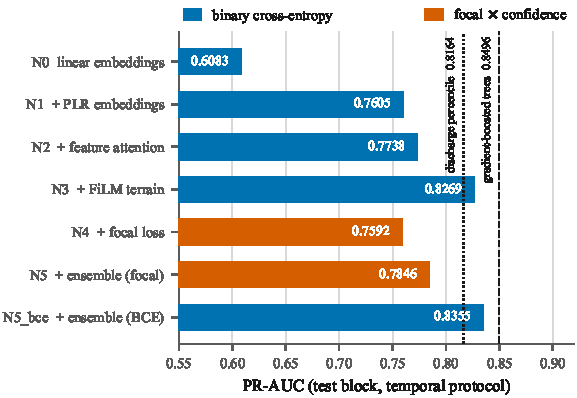
\includegraphics[width=\linewidth]{fig_ladder.pdf}
\caption{Test AP along the ablation sequence; marker shape shows the training
objective.}
\label{fig:ladder}
\end{figure}

\subsection{Radar fusion and model size}
Gated radar fusion raises the focal-loss ensemble from 0.785 to 0.831 but needs
about 17 times more parameters per member and still does not exceed the
image-free BCE model (0.836). Radar scalars alone reduce AP. With imagery at only
nine locations and a revisit of about twelve days against a one-day horizon,
the apparent radar gain mostly recovers what focal loss lost.

\subsection{Detection at operating points}
Fig.~\ref{fig:operating} shows episode detection against FAR. Configurations
with more alarms detect more episodes in advance: N2 detects 0.423 at FAR
0.313, whereas N3 and N5\_bce detect about 0.20--0.22 at FAR 0.11--0.12. Each
point uses its own threshold, so these are not a single operating curve.

\begin{figure}[t]
\centering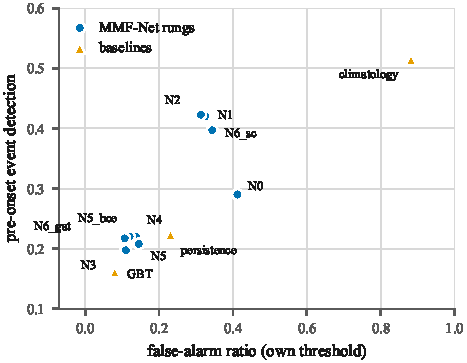
\includegraphics[width=\linewidth]{fig_operating_points.pdf}
\caption{Episode detection (alarm in the seven days before onset) against
node-day FAR for selected configurations.}
\label{fig:operating}
\end{figure}

%% =====================================================================
\section{Discussion}
The results support a simple design lesson: for tabular hydrometeorological
inputs, how a network reads each number matters more than adding recurrence,
graphs or imagery. PLR embeddings and FiLM account for most of the improvement,
and a plain BCE objective with ensembling and temperature scaling gives the most
trustworthy probabilities.

Several limitations bound these claims. The target is reanalysis discharge, not
measured water level or mapped inundation, so performance against gauges or
impacts is untested. Ablation steps N0--N4 are single-seed runs without
confidence intervals, the focal objective changes class weighting, focusing and
confidence weighting together, and ensembling and temperature scaling were
introduced jointly. Radar variants used the focal objective and limited
coverage, so they are not matched controls. Finally, operational inputs arrive
with delays that were not replayed here.

%% =====================================================================
\section{Conclusion and Future Work}
We presented \model{}, a terrain-conditioned transformer with periodic numerical
embeddings for next-day river high-flow forecasting across Sri Lanka. On held-out
future years it outperforms operational rules and our alternative graph-based
and compact architectures at every horizon and at flood onset, matches a
gradient-boosted tree at one day while leading at longer horizons and onset,
and delivers well-calibrated probabilities with far fewer false alarms. Future
work will evaluate against independent gauge and
inundation records, replay only data available at issue time, add confidence
intervals across seeds for every ablation, and test matched radar and graph
controls under the same objective.

%% =====================================================================
\balance
\begin{thebibliography}{00}
\bibitem{kratzert2018} F. Kratzert, D. Klotz, C. Brenner, K. Schulz, and
M. Herrnegger, ``Rainfall--runoff modelling using Long Short-Term Memory (LSTM)
networks,'' \emph{Hydrol. Earth Syst. Sci.}, vol. 22, pp. 6005--6022, 2018.
\bibitem{kratzert2019} F. Kratzert, D. Klotz, G. Shalev, G. Klambauer,
S. Hochreiter, and G. Nearing, ``Towards learning universal, regional, and local
hydrological behaviors via machine learning applied to large-sample datasets,''
\emph{Hydrol. Earth Syst. Sci.}, vol. 23, pp. 5089--5110, 2019.
\bibitem{nearing2024} G. Nearing \emph{et al.}, ``Global prediction of extreme
floods in ungauged watersheds,'' \emph{Nature}, vol. 627, pp. 559--563, 2024.
\bibitem{saubhagya2025} S. Saubhagya, C. Tilakaratne, P. Lakraj, and
M. Mammadov, ``A fusion of deep learning and time series regression for flood
forecasting: An application to the Ratnapura area based on the Kalu river basin
in Sri Lanka,'' \emph{Forecasting}, vol. 7, no. 2, art. 29, 2025.
\bibitem{thilakarathne2017} M. Thilakarathne and K. Premachandra, ``Predicting
floods in North Central Province of Sri Lanka using machine learning and data
mining methods,'' in \emph{Proc. SLAAI Int. Conf. Artificial Intelligence},
2017, pp. 44--49.
\bibitem{gunasekara2008} I. P. A. Gunasekara, ``Flood hazard mapping in lower
reach of Kelani river,'' \emph{ENGINEER}, vol. 41, no. 5, pp. 149--154, 2008.
\bibitem{mosavi2018} A. Mosavi, P. Ozturk, and K.-W. Chau, ``Flood prediction
using machine learning models: Literature review,'' \emph{Water}, vol. 10,
no. 11, art. 1536, 2018.
\bibitem{hochreiter1997} S. Hochreiter and J. Schmidhuber, ``Long short-term
memory,'' \emph{Neural Comput.}, vol. 9, no. 8, pp. 1735--1780, 1997.
\bibitem{vaswani2017} A. Vaswani \emph{et al.}, ``Attention is all you need,''
in \emph{Adv. Neural Inf. Process. Syst.}, vol. 30, 2017.
\bibitem{devlin2019} J. Devlin, M.-W. Chang, K. Lee, and K. Toutanova, ``BERT:
Pre-training of deep bidirectional transformers for language understanding,''
in \emph{Proc. NAACL-HLT}, 2019, pp. 4171--4186.
\bibitem{xiong2020} R. Xiong \emph{et al.}, ``On layer normalization in the
transformer architecture,'' in \emph{Proc. ICML}, PMLR vol. 119, 2020,
pp. 10524--10533.
\bibitem{ba2016} J. L. Ba, J. R. Kiros, and G. E. Hinton, ``Layer
normalization,'' arXiv:1607.06450, 2016.
\bibitem{hendrycks2016} D. Hendrycks and K. Gimpel, ``Gaussian error linear
units (GELUs),'' arXiv:1606.08415, 2016.
\bibitem{gorishniy2021} Y. Gorishniy, I. Rubachev, V. Khrulkov, and A. Babenko,
``Revisiting deep learning models for tabular data,'' in \emph{Adv. Neural Inf.
Process. Syst.}, vol. 34, 2021.
\bibitem{gorishniy2022} Y. Gorishniy, I. Rubachev, and A. Babenko, ``On
embeddings for numerical features in tabular deep learning,'' in \emph{Adv.
Neural Inf. Process. Syst.}, vol. 35, 2022.
\bibitem{tancik2020} M. Tancik \emph{et al.}, ``Fourier features let networks
learn high frequency functions in low dimensional domains,'' in \emph{Adv.
Neural Inf. Process. Syst.}, vol. 33, 2020.
\bibitem{grinsztajn2022} L. Grinsztajn, E. Oyallon, and G. Varoquaux, ``Why do
tree-based models still outperform deep learning on typical tabular data?'' in
\emph{Adv. Neural Inf. Process. Syst.}, vol. 35, 2022.
\bibitem{ke2017} G. Ke \emph{et al.}, ``LightGBM: A highly efficient gradient
boosting decision tree,'' in \emph{Adv. Neural Inf. Process. Syst.}, vol. 30,
2017.
\bibitem{lim2021} B. Lim, S. \"O. Ar{\i}k, N. Loeff, and T. Pfister, ``Temporal
fusion transformers for interpretable multi-horizon time series forecasting,''
\emph{Int. J. Forecast.}, vol. 37, no. 4, pp. 1748--1764, 2021.
\bibitem{perez2018} E. Perez, F. Strub, H. de Vries, V. Dumoulin, and
A. Courville, ``FiLM: Visual reasoning with a general conditioning layer,''
in \emph{Proc. AAAI}, vol. 32, no. 1, 2018.
\bibitem{kirschstein2024} N. Kirschstein and Y. Sun, ``The merit of river
network topology for neural flood forecasting,'' in \emph{Proc. ICML},
PMLR vol. 235, 2024, pp. 24713--24725.
\bibitem{he2016} K. He, X. Zhang, S. Ren, and J. Sun, ``Deep residual learning
for image recognition,'' in \emph{Proc. CVPR}, 2016, pp. 770--778.
\bibitem{torres2012} R. Torres \emph{et al.}, ``GMES Sentinel-1 mission,''
\emph{Remote Sens. Environ.}, vol. 120, pp. 9--24, 2012.
\bibitem{lin2017} T.-Y. Lin, P. Goyal, R. Girshick, K. He, and P. Doll\'{a}r,
``Focal loss for dense object detection,'' in \emph{Proc. ICCV}, 2017,
pp. 2980--2988.
\bibitem{huber1964} P. J. Huber, ``Robust estimation of a location
parameter,'' \emph{Ann. Math. Stat.}, vol. 35, no. 1, pp. 73--101, 1964.
\bibitem{lakshminarayanan2017} B. Lakshminarayanan, A. Pritzel, and C. Blundell,
``Simple and scalable predictive uncertainty estimation using deep ensembles,''
in \emph{Adv. Neural Inf. Process. Syst.}, vol. 30, 2017.
\bibitem{guo2017} C. Guo, G. Pleiss, Y. Sun, and K. Q. Weinberger, ``On
calibration of modern neural networks,'' in \emph{Proc. ICML}, PMLR vol. 70,
2017, pp. 1321--1330.
\bibitem{naeini2015} M. P. Naeini, G. F. Cooper, and M. Hauskrecht, ``Obtaining
well calibrated probabilities using Bayesian binning,'' in \emph{Proc. AAAI},
2015, pp. 2901--2907.
\bibitem{saito2015} T. Saito and M. Rehmsmeier, ``The precision-recall plot is
more informative than the ROC plot when evaluating binary classifiers on
imbalanced datasets,'' \emph{PLOS ONE}, vol. 10, no. 3, art. e0118432, 2015.
\bibitem{brier1950} G. W. Brier, ``Verification of forecasts expressed in terms
of probability,'' \emph{Mon. Weather Rev.}, vol. 78, no. 1, pp. 1--3, 1950.
\bibitem{jolliffe2012} I. T. Jolliffe and D. B. Stephenson, Eds., \emph{Forecast
Verification: A Practitioner's Guide in Atmospheric Science}, 2nd ed.
Chichester, U.K.: Wiley, 2012.
\bibitem{roberts2017} D. R. Roberts \emph{et al.}, ``Cross-validation strategies
for data with temporal, spatial, hierarchical, or phylogenetic structure,''
\emph{Ecography}, vol. 40, no. 8, pp. 913--929, 2017.
\bibitem{kapoor2023} S. Kapoor and A. Narayanan, ``Leakage and the
reproducibility crisis in machine-learning-based science,'' \emph{Patterns},
vol. 4, no. 9, art. 100804, 2023.
\bibitem{paszke2019} A. Paszke \emph{et al.}, ``PyTorch: An imperative style,
high-performance deep learning library,'' in \emph{Adv. Neural Inf. Process.
Syst.}, vol. 32, 2019.
\bibitem{loshchilov2019} I. Loshchilov and F. Hutter, ``Decoupled weight decay
regularization,'' in \emph{Proc. ICLR}, 2019.
\bibitem{power} NASA POWER, ``Meteorology: Data sources and methodology.''
[Online]. Available: \url{https://power.larc.nasa.gov/docs/methodology/meteorology/}
\bibitem{munoz2021} J. Mu\~noz-Sabater \emph{et al.}, ``ERA5-Land: A
state-of-the-art global reanalysis dataset for land applications,''
\emph{Earth Syst. Sci. Data}, vol. 13, pp. 4349--4383, 2021.
\bibitem{harrigan2020} S. Harrigan \emph{et al.}, ``GloFAS-ERA5 operational
global river discharge reanalysis 1979--present,'' \emph{Earth Syst. Sci. Data},
vol. 12, pp. 2043--2060, 2020.
\bibitem{openmeteo} Open-Meteo, ``Flood API.'' [Online]. Available:
\url{https://open-meteo.com/en/docs/flood-api}
\end{thebibliography}
\end{document}
